\documentclass{standalone}
\usepackage{tikz}
\usetikzlibrary{patterns, positioning}
\usepackage[sfdefault]{ClearSans} %% option 'sfdefault' activates Clear Sans as the default text font
\usepackage[T1]{fontenc}

\begin{document}
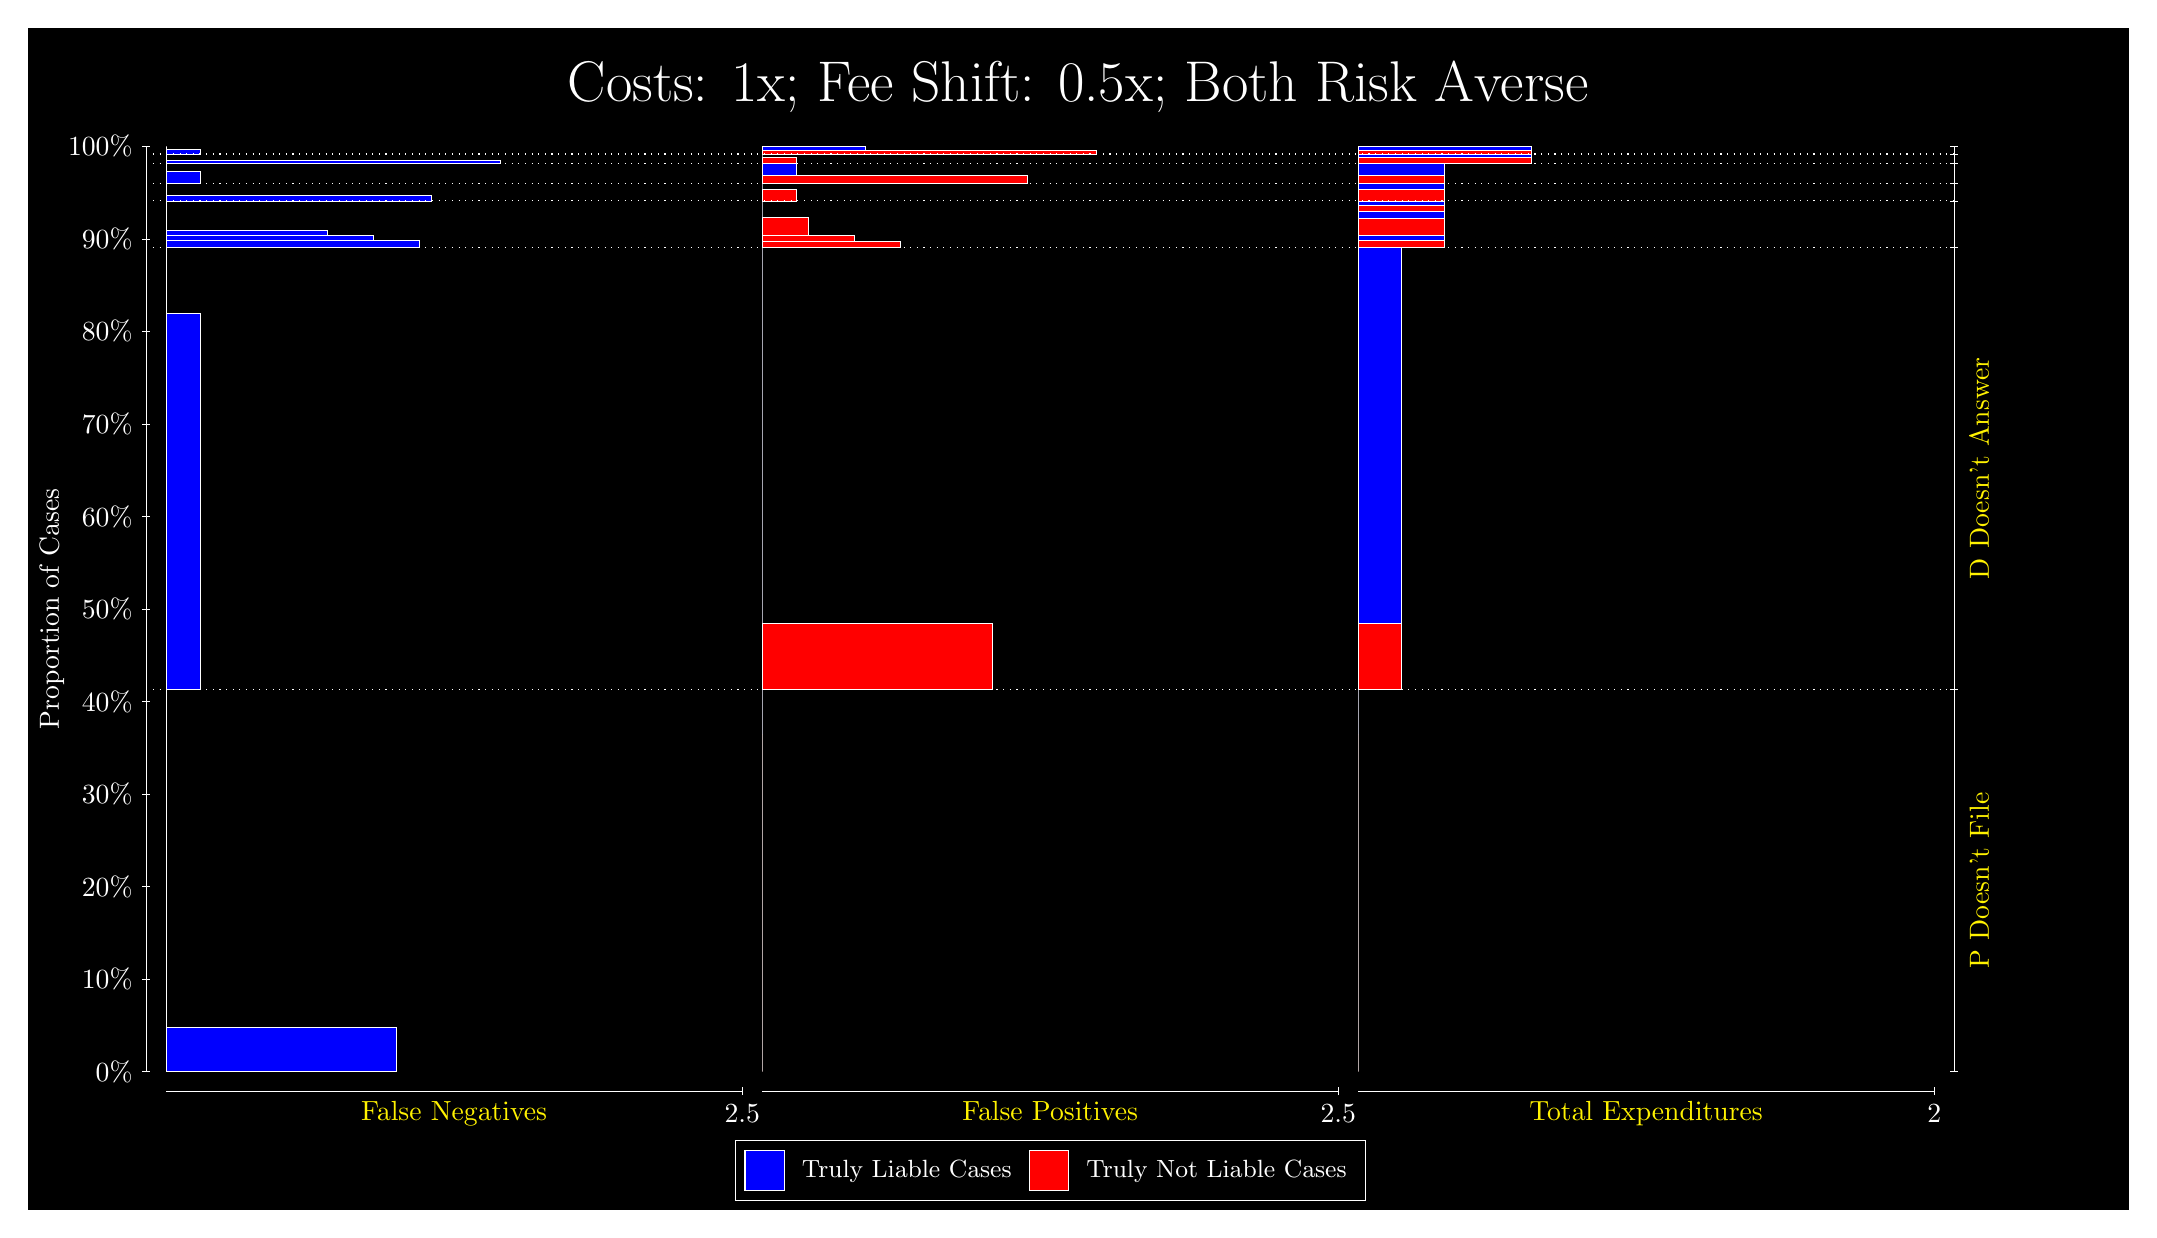
\begin{tikzpicture}
\draw[fill=black] (0,0) rectangle (26.667,15);
\draw[text=white] (0,13.5) rectangle (26.667,15) node[midway] {\huge Costs: 1x; Fee Shift: 0.5x; Both Risk Averse};
\draw[white, very thin] (1.5,1.75) -- (1.5,13.5);
\node[rotate=90, text=white, anchor=center] at (0.3, 7.625) {Proportion of Cases};
\draw[white, very thin] (1.45,1.75) -- (1.55,1.75);
\node[text=white, anchor=east] at (1.45, 1.75) {0\%};
\draw[white, very thin] (1.45,2.925) -- (1.55,2.925);
\node[text=white, anchor=east] at (1.45, 2.925) {10\%};
\draw[white, very thin] (1.45,4.1) -- (1.55,4.1);
\node[text=white, anchor=east] at (1.45, 4.1) {20\%};
\draw[white, very thin] (1.45,5.275) -- (1.55,5.275);
\node[text=white, anchor=east] at (1.45, 5.275) {30\%};
\draw[white, very thin] (1.45,6.45) -- (1.55,6.45);
\node[text=white, anchor=east] at (1.45, 6.45) {40\%};
\draw[white, very thin] (1.45,7.625) -- (1.55,7.625);
\node[text=white, anchor=east] at (1.45, 7.625) {50\%};
\draw[white, very thin] (1.45,8.8) -- (1.55,8.8);
\node[text=white, anchor=east] at (1.45, 8.8) {60\%};
\draw[white, very thin] (1.45,9.975) -- (1.55,9.975);
\node[text=white, anchor=east] at (1.45, 9.975) {70\%};
\draw[white, very thin] (1.45,11.15) -- (1.55,11.15);
\node[text=white, anchor=east] at (1.45, 11.15) {80\%};
\draw[white, very thin] (1.45,12.325) -- (1.55,12.325);
\node[text=white, anchor=east] at (1.45, 12.325) {90\%};
\draw[white, very thin] (1.45,13.5) -- (1.55,13.5);
\node[text=white, anchor=east] at (1.45, 13.5) {100\%};

\draw[white, very thin] (24.457,1.75) -- (24.457,13.5);
\draw[white, very thin] (24.407,1.75) -- (24.507,1.75);
\node[anchor=west] at (24.407, 1.75) {};
\draw[white, very thin] (24.407,6.6031) -- (24.507,6.6031);
\node[anchor=west] at (24.407, 6.6031) {};
\draw[white, very thin] (24.407,12.217) -- (24.507,12.217);
\node[anchor=west] at (24.407, 12.217) {};
\draw[white, very thin] (24.407,12.807) -- (24.507,12.807);
\node[anchor=west] at (24.407, 12.807) {};
\draw[white, very thin] (24.407,13.03) -- (24.507,13.03);
\node[anchor=west] at (24.407, 13.03) {};
\draw[white, very thin] (24.407,13.281) -- (24.507,13.281);
\node[anchor=west] at (24.407, 13.281) {};
\draw[white, very thin] (24.407,13.402) -- (24.507,13.402);
\node[anchor=west] at (24.407, 13.402) {};
\draw[white, very thin] (24.407,13.5) -- (24.507,13.5);
\node[anchor=west] at (24.407, 13.5) {};

\draw[white, very thin, fill=blue] (1.75,1.75) rectangle (4.6775,2.3168);
\draw[white, very thin, fill=red] (1.75,2.3168) rectangle (1.75,6.6031);
\draw[white, very thin, fill=blue] (1.75,6.6031) rectangle (2.1891,11.375);
\draw[white, very thin, fill=red] (1.75,11.375) rectangle (1.75,12.217);
\draw[white, very thin, fill=blue] (1.75,12.217) rectangle (4.9703,12.307);
\draw[white, very thin, fill=blue] (1.75,12.307) rectangle (4.3848,12.367);
\draw[white, very thin, fill=blue] (1.75,12.367) rectangle (3.7993,12.429);
\draw[white, very thin, fill=red] (1.75,12.429) rectangle (1.75,12.807);
\draw[white, very thin, fill=blue] (1.75,12.807) rectangle (5.1167,12.881);
\draw[white, very thin, fill=red] (1.75,12.881) rectangle (1.75,13.03);
\draw[white, very thin, fill=blue] (1.75,13.03) rectangle (2.1891,13.177);
\draw[white, very thin, fill=red] (1.75,13.177) rectangle (1.75,13.281);
\draw[white, very thin, fill=blue] (1.75,13.281) rectangle (5.9949,13.327);
\draw[white, very thin, fill=red] (1.75,13.327) rectangle (1.75,13.402);
\draw[white, very thin, fill=blue] (1.75,13.402) rectangle (2.1891,13.458);
\draw[white, very thin, fill=red] (1.75,13.458) rectangle (1.75,13.5);
\draw[white, very thin, fill=red] (9.3189,1.75) rectangle (9.3189,6.0363);
\draw[white, very thin, fill=blue] (9.3189,6.0363) rectangle (9.3189,6.6031);
\draw[white, very thin, fill=red] (9.3189,6.6031) rectangle (12.246,7.4444);
\draw[white, very thin, fill=blue] (9.3189,7.4444) rectangle (9.3189,12.217);
\draw[white, very thin, fill=red] (9.3189,12.217) rectangle (11.075,12.29);
\draw[white, very thin, fill=red] (9.3189,12.29) rectangle (10.49,12.376);
\draw[white, very thin, fill=red] (9.3189,12.376) rectangle (9.9044,12.595);
\draw[white, very thin, fill=blue] (9.3189,12.595) rectangle (9.3189,12.807);
\draw[white, very thin, fill=red] (9.3189,12.807) rectangle (9.758,12.956);
\draw[white, very thin, fill=blue] (9.3189,12.956) rectangle (9.3189,13.03);
\draw[white, very thin, fill=red] (9.3189,13.03) rectangle (12.686,13.134);
\draw[white, very thin, fill=blue] (9.3189,13.134) rectangle (9.758,13.281);
\draw[white, very thin, fill=red] (9.3189,13.281) rectangle (9.758,13.356);
\draw[white, very thin, fill=blue] (9.3189,13.356) rectangle (9.3189,13.402);
\draw[white, very thin, fill=red] (9.3189,13.402) rectangle (13.564,13.444);
\draw[white, very thin, fill=blue] (9.3189,13.444) rectangle (10.636,13.5);
\draw[white, very thin, fill=red] (16.888,1.75) rectangle (16.888,6.0363);
\draw[white, very thin, fill=blue] (16.888,6.0363) rectangle (16.888,6.6031);
\draw[white, very thin, fill=red] (16.888,6.6031) rectangle (17.437,7.4444);
\draw[white, very thin, fill=blue] (16.888,7.4444) rectangle (17.437,12.217);
\draw[white, very thin, fill=red] (16.888,12.217) rectangle (17.986,12.303);
\draw[white, very thin, fill=blue] (16.888,12.303) rectangle (17.986,12.364);
\draw[white, very thin, fill=red] (16.888,12.364) rectangle (17.986,12.582);
\draw[white, very thin, fill=blue] (16.888,12.582) rectangle (17.986,12.672);
\draw[white, very thin, fill=red] (16.888,12.672) rectangle (17.986,12.745);
\draw[white, very thin, fill=blue] (16.888,12.745) rectangle (17.986,12.807);
\draw[white, very thin, fill=red] (16.888,12.807) rectangle (17.986,12.956);
\draw[white, very thin, fill=blue] (16.888,12.956) rectangle (17.986,13.03);
\draw[white, very thin, fill=red] (16.888,13.03) rectangle (17.986,13.134);
\draw[white, very thin, fill=blue] (16.888,13.134) rectangle (17.986,13.281);
\draw[white, very thin, fill=red] (16.888,13.281) rectangle (19.083,13.356);
\draw[white, very thin, fill=blue] (16.888,13.356) rectangle (19.083,13.402);
\draw[white, very thin, fill=red] (16.888,13.402) rectangle (19.083,13.444);
\draw[white, very thin, fill=blue] (16.888,13.444) rectangle (19.083,13.5);
\draw[white, dotted] (1.5,6.6031) -- (24.457,6.6031);
\draw[white, dotted] (1.5,12.217) -- (24.457,12.217);
\draw[white, dotted] (1.5,12.807) -- (24.457,12.807);
\draw[white, dotted] (1.5,13.03) -- (24.457,13.03);
\draw[white, dotted] (1.5,13.281) -- (24.457,13.281);
\draw[white, dotted] (1.5,13.402) -- (24.457,13.402);
\draw[white, very thin] (1.75,1.5) -- (9.0689,1.5);
\node[text=yellow, anchor=north] at (5.4094, 1.5) {False Negatives};
\draw[white, very thin] (9.0689,1.45) -- (9.0689,1.55);
\node[text=white, anchor=north] at (9.0689, 1.45) {2.5};

\draw[white, very thin] (9.3189,1.5) -- (16.638,1.5);
\node[text=yellow, anchor=north] at (12.978, 1.5) {False Positives};
\draw[white, very thin] (16.638,1.45) -- (16.638,1.55);
\node[text=white, anchor=north] at (16.638, 1.45) {2.5};

\draw[white, very thin] (16.888,1.5) -- (24.207,1.5);
\node[text=yellow, anchor=north] at (20.547, 1.5) {Total Expenditures};
\draw[white, very thin] (24.207,1.45) -- (24.207,1.55);
\node[text=white, anchor=north] at (24.207, 1.45) {2};

\node[text=yellow, centered, rotate=90] at (24.777, 4.1766) {P Doesn't File};
\node[text=yellow, centered, rotate=90] at (24.777, 9.4099) {D Doesn't Answer};






\draw (12.978300999999998,1.5) node[draw=none] (baseCoordinate) {};
\begin{scope}[align=center]
        \matrix[scale=0.5, draw=white, below=0.5cm of baseCoordinate, nodes={draw}, column sep=0.1cm]{
            \node[rectangle, draw, minimum width=0.5cm, minimum height=0.5cm, fill=blue] {}; &
            \node[draw=none, font=\small, text=white] (B) {Truly Liable Cases}; &
            \node[rectangle, draw, minimum width=0.5cm, minimum height=0.5cm, fill=red] {}; &
            \node[draw=none, font=\small, text=white] (B) {Truly Not Liable Cases}; \\
            };
\end{scope}

\end{tikzpicture}
\end{document}